\documentclass[11pt,a4paper]{article}

\usepackage[margin=0.85in]{geometry}
\usepackage[T1]{fontenc}
\usepackage{lmodern}
\usepackage{xcolor}
\usepackage{amsmath,amssymb}
\usepackage{booktabs}
\usepackage{array}
\usepackage{tcolorbox}
\usepackage{tikz}
\usepackage{pgfplots}
\usepackage{listings}
\usepackage{hyperref}
\usepackage{enumitem}
\usepackage{caption}
\usepackage{microtype}

\usetikzlibrary{arrows.meta,positioning,calc,shapes.geometric,fit,backgrounds}
\pgfplotsset{compat=1.18}

\definecolor{ink}{HTML}{17212B}
\definecolor{muted}{HTML}{5D6B78}
\definecolor{sky}{HTML}{2F80ED}
\definecolor{teal}{HTML}{0E9F8F}
\definecolor{sun}{HTML}{F2A900}
\definecolor{coral}{HTML}{E85D75}
\definecolor{leaf}{HTML}{27AE60}
\definecolor{paper}{HTML}{FAFBFC}
\definecolor{panel}{HTML}{EEF6FF}
\definecolor{codebg}{HTML}{F6F8FA}
\definecolor{obstacle}{HTML}{2E3440}
\definecolor{gridline}{HTML}{D5DEE8}

\hypersetup{
  colorlinks=true,
  linkcolor=sky,
  urlcolor=teal,
  citecolor=sky
}

\lstdefinestyle{pythonstyle}{
  language=Python,
  backgroundcolor=\color{codebg},
  basicstyle=\ttfamily\small,
  keywordstyle=\color{sky}\bfseries,
  stringstyle=\color{leaf},
  commentstyle=\color{muted}\itshape,
  numberstyle=\tiny\color{muted},
  numbers=left,
  stepnumber=1,
  numbersep=8pt,
  showstringspaces=false,
  breaklines=true,
  frame=single,
  rulecolor=\color{gridline},
  tabsize=4,
  columns=fullflexible
}

\tcbset{
  colback=paper,
  colframe=sky!50!black,
  arc=2mm,
  boxrule=0.6pt,
  left=8pt,
  right=8pt,
  top=7pt,
  bottom=7pt
}

\newtcolorbox{bigidea}[1]{
  title=\textbf{#1},
  colback=panel,
  colframe=sky,
  fonttitle=\large
}

\newtcolorbox{gentle}[1]{
  title=\textbf{#1},
  colback=teal!6,
  colframe=teal!70!black
}

\newcommand{\nodecircle}[4]{
  \node[circle,draw=#3,fill=#3!12,minimum size=9mm,thick] (#1) at #2 {\small #4};
}

\title{\Huge\bfseries Dijkstra and A* for Robotics\\[4pt]
\Large A Gentle, Visual Path-Planning Guide}
\author{Made for learning from zero: concept $\rightarrow$ math $\rightarrow$ Python}
\date{}

\begin{document}
\maketitle

\begin{center}
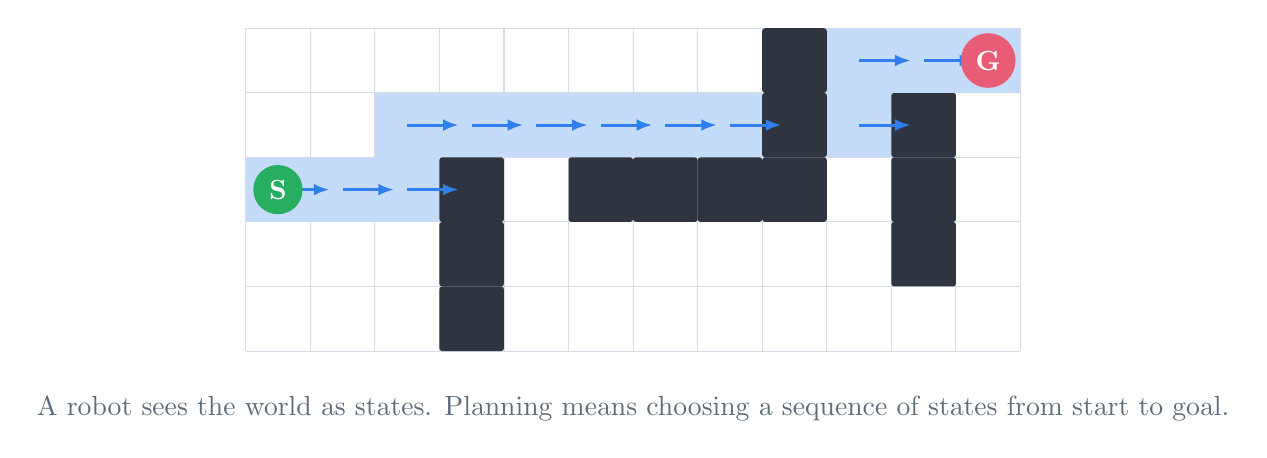
\begin{tikzpicture}[scale=0.82]
  \draw[step=1, color=gridline] (0,0) grid (12,5);
  \foreach \x/\y in {3/0,3/1,3/2,5/2,6/2,7/2,8/2,8/3,8/4,10/1,10/2,10/3}
    \fill[obstacle, rounded corners=1pt] (\x,\y) rectangle ++(1,1);
  \foreach \x/\y in {0/2,1/2,2/2,2/3,3/3,4/3,5/3,6/3,7/3,9/3,9/4,10/4,11/4}
    \fill[sky!28] (\x,\y) rectangle ++(1,1);
  \foreach \x/\y in {0/2,1/2,2/2,2/3,3/3,4/3,5/3,6/3,7/3,9/3,9/4,10/4}
    \draw[-{Latex[length=2mm]}, sky, line width=1.1pt] (\x+0.5,\y+0.5) -- ++(0.8,0);
  \node[circle,fill=leaf,text=white,inner sep=3pt] at (0.5,2.5) {\textbf{S}};
  \node[circle,fill=coral,text=white,inner sep=3pt] at (11.5,4.5) {\textbf{G}};
  \node[below=8pt, text=muted] at (6,-0.2) {A robot sees the world as states. Planning means choosing a sequence of states from start to goal.};
\end{tikzpicture}
\end{center}

\tableofcontents
\newpage

\section{Concept First: What Problem Are We Solving?}

\begin{bigidea}{The path-planning question}
A robot is at a start position. It needs to reach a goal position. Some places are blocked, some motions are expensive, and the robot should choose a path that is valid and cheap.
\end{bigidea}

In robotics, we often convert the world into a \textbf{graph}.

\begin{itemize}[leftmargin=*]
  \item A \textbf{node} is a possible robot state: a grid cell, a room, a road point, or even a full pose $(x,y,\theta)$.
  \item An \textbf{edge} is a possible movement from one state to another.
  \item A \textbf{cost} is how expensive that movement is: distance, time, energy, risk, or a mixture of these.
\end{itemize}

\begin{center}
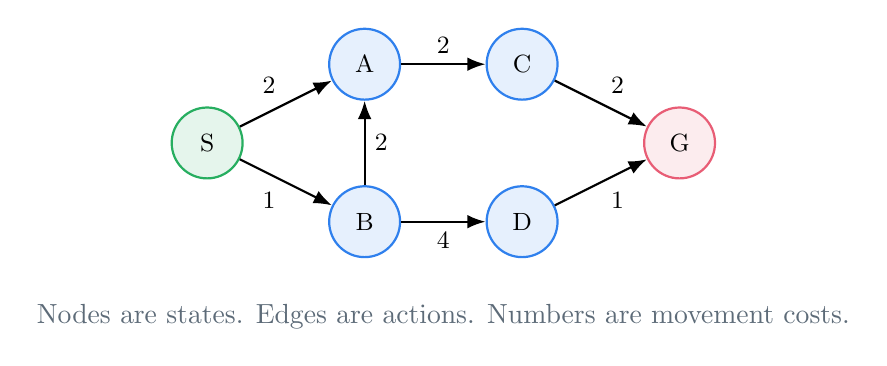
\begin{tikzpicture}[node distance=18mm,>=Latex]
  \nodecircle{A}{(0,0)}{leaf}{S}
  \nodecircle{B}{(2,1)}{sky}{A}
  \nodecircle{C}{(2,-1)}{sky}{B}
  \nodecircle{D}{(4,1)}{sky}{C}
  \nodecircle{E}{(4,-1)}{sky}{D}
  \nodecircle{F}{(6,0)}{coral}{G}
  \draw[->,thick] (A) -- node[above left] {\small 2} (B);
  \draw[->,thick] (A) -- node[below left] {\small 1} (C);
  \draw[->,thick] (B) -- node[above] {\small 2} (D);
  \draw[->,thick] (C) -- node[below] {\small 4} (E);
  \draw[->,thick] (C) -- node[right] {\small 2} (B);
  \draw[->,thick] (D) -- node[above right] {\small 2} (F);
  \draw[->,thick] (E) -- node[below right] {\small 1} (F);
  \node[text=muted,align=center] at (3,-2.2) {Nodes are states. Edges are actions. Numbers are movement costs.};
\end{tikzpicture}
\end{center}

\subsection{What Dijkstra Does}

Dijkstra's algorithm is like pouring water from the start. The water spreads outward in order of cheapest known distance. The first time the water reaches the goal, the route is guaranteed to be shortest, as long as all edge costs are non-negative.

\begin{gentle}{Dijkstra in one sentence}
Always expand the not-yet-expanded node with the smallest known cost from the start.
\end{gentle}

\subsection{What A* Does}

A* is Dijkstra with a sense of direction. It still tracks the cost already paid, but it also estimates how far a node is from the goal. This estimate is called a \textbf{heuristic}.

\begin{gentle}{A* in one sentence}
Always expand the node that looks cheapest by combining cost already paid and estimated cost still remaining.
\end{gentle}

\begin{center}
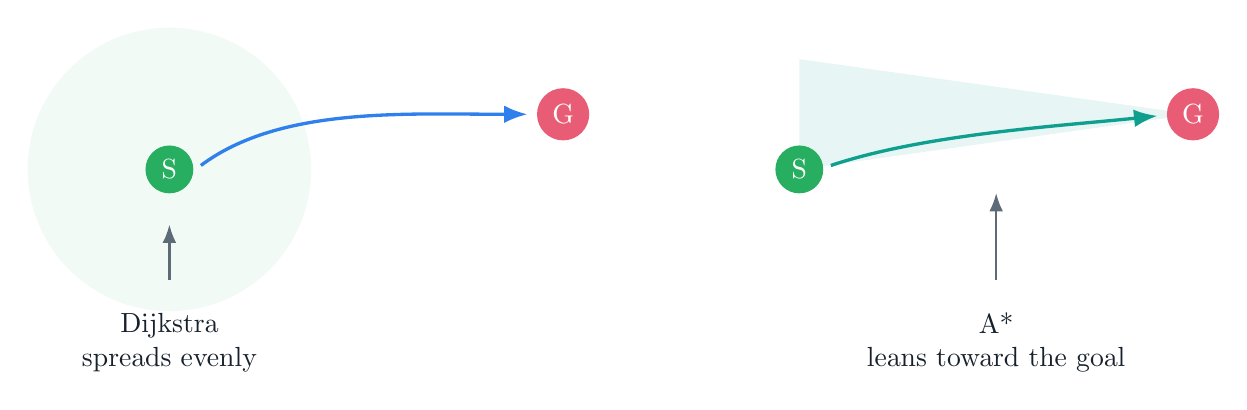
\begin{tikzpicture}[scale=1,>=Latex]
  \fill[leaf!15] (0,0) circle (0.6);
  \fill[leaf!10] (0,0) circle (1.2);
  \fill[leaf!6] (0,0) circle (1.8);
  \node[circle,fill=leaf,text=white,inner sep=3pt] at (0,0) {S};
  \node[circle,fill=coral,text=white,inner sep=3pt] at (5,0.7) {G};
  \draw[-{Latex[length=3mm]}, sky, very thick] (0.4,0.05) .. controls (1.4,0.8) and (3,0.7) .. (4.55,0.7);
  \node[align=center,text=ink] at (0,-2.2) {Dijkstra\\spreads evenly};
  \draw[->,thick,muted] (0,-1.4) -- (0,-0.7);

  \begin{scope}[xshift=8cm]
    \fill[teal!10] (0,0) -- (5,0.7) -- (0,1.4) -- cycle;
    \node[circle,fill=leaf,text=white,inner sep=3pt] at (0,0) {S};
    \node[circle,fill=coral,text=white,inner sep=3pt] at (5,0.7) {G};
    \draw[-{Latex[length=3mm]}, teal, very thick] (0.4,0.05) .. controls (1.6,0.45) and (3.3,0.55) .. (4.55,0.68);
    \node[align=center,text=ink] at (2.5,-2.2) {A*\\leans toward the goal};
    \draw[->,thick,muted] (2.5,-1.4) -- (2.5,-0.3);
  \end{scope}
\end{tikzpicture}
\end{center}

\section{Robotics View: From Map to Graph}

For a beginner, the cleanest robotics example is a \textbf{grid map}. Imagine a small mobile robot moving on square cells.

\begin{itemize}[leftmargin=*]
  \item White cells are free.
  \item Dark cells are obstacles.
  \item The robot can move up, down, left, and right.
  \item Each move costs $1$.
\end{itemize}

\begin{center}
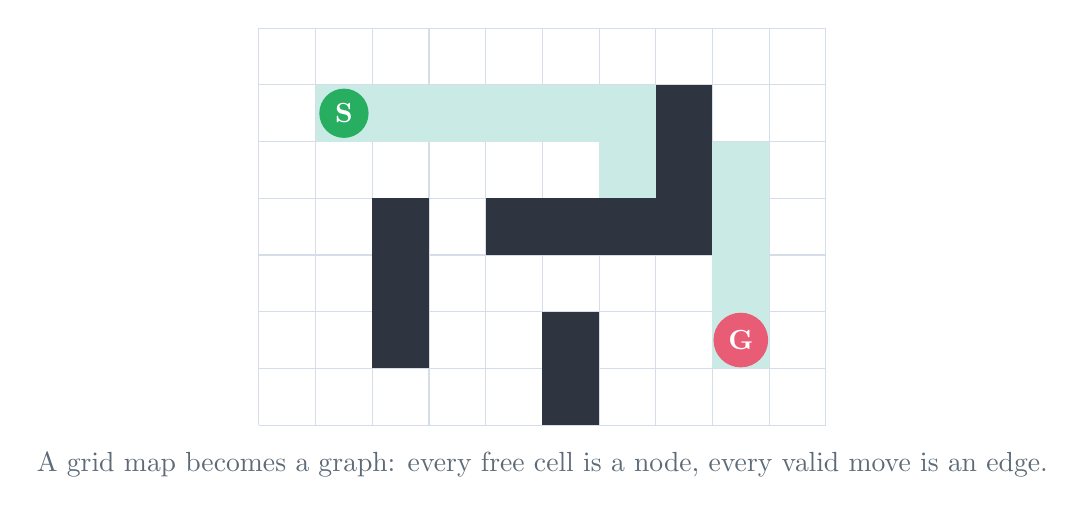
\begin{tikzpicture}[scale=0.72]
  \draw[step=1, color=gridline] (0,0) grid (10,7);
  \foreach \x/\y in {2/1,2/2,2/3,4/3,5/3,6/3,7/3,7/4,7/5,5/0,5/1}
    \fill[obstacle] (\x,\y) rectangle ++(1,1);
  \foreach \x/\y in {1/5,2/5,3/5,4/5,5/5,6/5,6/4,8/4,8/3,8/2,8/1}
    \fill[teal!22] (\x,\y) rectangle ++(1,1);
  \node[circle,fill=leaf,text=white,inner sep=3pt] at (1.5,5.5) {\textbf{S}};
  \node[circle,fill=coral,text=white,inner sep=3pt] at (8.5,1.5) {\textbf{G}};
  \node[text=muted,align=center] at (5,-0.7) {A grid map becomes a graph: every free cell is a node, every valid move is an edge.};
\end{tikzpicture}
\end{center}

This grid is a simplification. Real robots may need continuous motion, turning radius, collision checking, localization uncertainty, dynamic obstacles, and speed limits. But Dijkstra and A* remain foundational because many advanced planners are built on the same idea: search through possible states while keeping track of cost.

\section{The Mathematics, Gently}

\subsection{Graph Model}

We describe the planning problem as a weighted graph:

\[
G = (V, E)
\]

\begin{itemize}[leftmargin=*]
  \item $V$ is the set of vertices, also called nodes or states.
  \item $E$ is the set of edges, also called actions or transitions.
  \item Each edge $(u,v)$ has a cost $w(u,v)$.
\end{itemize}

For shortest-path planning, we want:

\[
\text{best path} = \arg\min_{\text{paths } P:s\to g} \sum_{(u,v)\in P} w(u,v)
\]

In plain English: among all paths from start $s$ to goal $g$, choose the path whose total movement cost is smallest.

\subsection{Dijkstra's Score}

Dijkstra keeps a value:

\[
d(n) = \text{best cost found so far from start } s \text{ to node } n
\]

At the start:

\[
d(s)=0,\qquad d(n)=\infty \text{ for every other node}
\]

When Dijkstra sees that it can go from $u$ to $v$, it asks:

\[
\text{new cost to } v = d(u) + w(u,v)
\]

If this is better than the old value:

\[
d(u)+w(u,v) < d(v)
\]

then update:

\[
d(v) \leftarrow d(u)+w(u,v)
\]

This update is called \textbf{relaxation}. The word sounds fancy, but it simply means: ``I found a cheaper way to reach this node.''

\begin{center}
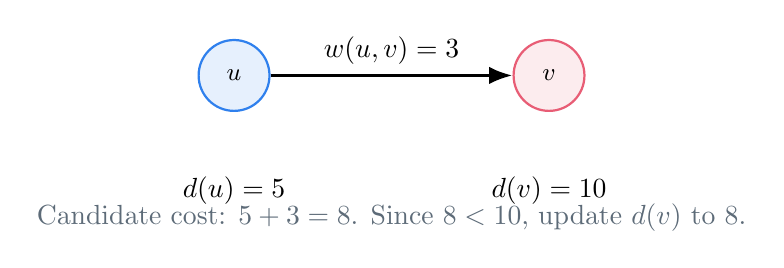
\begin{tikzpicture}[>=Latex]
  \nodecircle{u}{(0,0)}{sky}{$u$}
  \nodecircle{v}{(4,0)}{coral}{$v$}
  \draw[->,very thick] (u) -- node[above] {$w(u,v)=3$} (v);
  \node[below=7mm of u] {$d(u)=5$};
  \node[below=7mm of v] {$d(v)=10$};
  \node[align=center,text=muted] at (2,-1.8) {Candidate cost: $5+3=8$. Since $8<10$, update $d(v)$ to $8$.};
\end{tikzpicture}
\end{center}

\subsection{A* Score}

A* uses two costs:

\[
g(n) = \text{cost already paid from start to } n
\]

\[
h(n) = \text{estimated cost from } n \text{ to the goal}
\]

Then A* ranks nodes by:

\[
f(n) = g(n) + h(n)
\]

\begin{center}
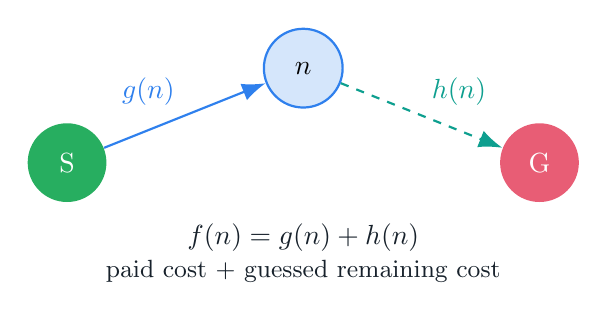
\begin{tikzpicture}[>=Latex]
  \node[circle,fill=leaf,text=white,minimum size=10mm] (s) at (0,0) {S};
  \node[circle,fill=sky!20,draw=sky,thick,minimum size=10mm] (n) at (3,1.2) {$n$};
  \node[circle,fill=coral,text=white,minimum size=10mm] (g) at (6,0) {G};
  \draw[-{Latex[length=3mm]},thick,sky] (s) -- node[above left] {$g(n)$} (n);
  \draw[-{Latex[length=3mm]},thick,teal,dashed] (n) -- node[above right] {$h(n)$} (g);
  \node[align=center,text=ink] at (3,-1.15) {$f(n)=g(n)+h(n)$\\\small paid cost + guessed remaining cost};
\end{tikzpicture}
\end{center}

\subsection{Common Heuristics for Robot Grids}

The heuristic should be easy to compute and should not overestimate the real cheapest remaining cost if you want guaranteed optimality.

\begin{center}
\begin{tabular}{>{\raggedright\arraybackslash}p{0.25\linewidth} >{\raggedright\arraybackslash}p{0.35\linewidth} >{\raggedright\arraybackslash}p{0.28\linewidth}}
\toprule
\textbf{Heuristic} & \textbf{Formula} & \textbf{Use when}\\
\midrule
Manhattan & $|x_1-x_2|+|y_1-y_2|$ & Robot moves only 4 directions.\\
Euclidean & $\sqrt{(x_1-x_2)^2+(y_1-y_2)^2}$ & Robot can move freely or diagonally.\\
Chebyshev & $\max(|x_1-x_2|,|y_1-y_2|)$ & Diagonal moves cost the same as straight moves.\\
\bottomrule
\end{tabular}
\end{center}

\begin{bigidea}{Why A* can be faster}
Dijkstra asks, ``What is the cheapest node I know how to reach?'' A* asks, ``What is the cheapest node if I include a reasonable guess toward the goal?''
\end{bigidea}

\subsection{Admissible and Consistent Heuristics}

A heuristic is \textbf{admissible} if it never overestimates:

\[
h(n) \le h^*(n)
\]

where $h^*(n)$ is the true shortest remaining cost from $n$ to the goal.

A heuristic is \textbf{consistent} if:

\[
h(u) \le w(u,v) + h(v)
\]

for every edge $(u,v)$. Consistency means the heuristic behaves like a real distance: going from $u$ to $v$ and then estimating from $v$ should not magically become more expensive than estimating from $u$ directly.

\begin{gentle}{Beginner mental model}
If the heuristic is too optimistic, A* may explore extra nodes but still finds the best path. If the heuristic is too aggressive and overestimates, A* may become faster but can miss the true shortest path.
\end{gentle}

\section{Step-by-Step Dijkstra Example}

Consider this tiny graph:

\begin{center}
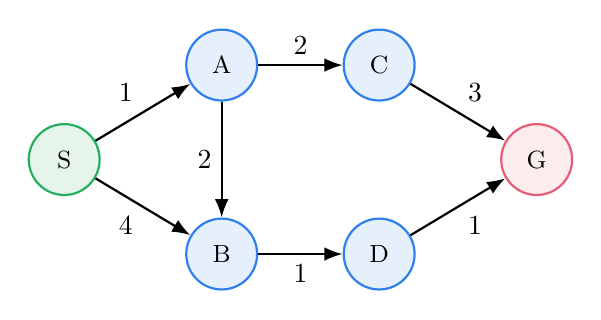
\begin{tikzpicture}[>=Latex]
  \nodecircle{S}{(0,0)}{leaf}{S}
  \nodecircle{A}{(2,1.2)}{sky}{A}
  \nodecircle{B}{(2,-1.2)}{sky}{B}
  \nodecircle{C}{(4,1.2)}{sky}{C}
  \nodecircle{D}{(4,-1.2)}{sky}{D}
  \nodecircle{G}{(6,0)}{coral}{G}
  \draw[->,thick] (S) -- node[above left] {1} (A);
  \draw[->,thick] (S) -- node[below left] {4} (B);
  \draw[->,thick] (A) -- node[above] {2} (C);
  \draw[->,thick] (A) -- node[left] {2} (B);
  \draw[->,thick] (B) -- node[below] {1} (D);
  \draw[->,thick] (C) -- node[above right] {3} (G);
  \draw[->,thick] (D) -- node[below right] {1} (G);
\end{tikzpicture}
\end{center}

\begin{center}
\begin{tabular}{c c c c}
\toprule
\textbf{Step} & \textbf{Expand} & \textbf{Known distances after update} & \textbf{Why}\\
\midrule
0 & none & $d(S)=0$, others $\infty$ & Start has zero cost.\\
1 & S & $d(A)=1$, $d(B)=4$ & From S, A is cheaper than B.\\
2 & A & $d(C)=3$, $d(B)=3$ & B improves via A: $1+2=3$.\\
3 & B & $d(D)=4$ & D reached with $3+1=4$.\\
4 & C & $d(G)=6$ & G reached with $3+3=6$.\\
5 & D & $d(G)=5$ & G improves via D: $4+1=5$.\\
\bottomrule
\end{tabular}
\end{center}

The best path is:

\[
S \rightarrow A \rightarrow B \rightarrow D \rightarrow G
\]

with total cost:

\[
1+2+1+1=5
\]

\section{Python Code: Dijkstra on a Graph}

\begin{lstlisting}[style=pythonstyle]
import heapq


def dijkstra(graph, start, goal):
    """
    graph example:
    {
        "S": [("A", 1), ("B", 4)],
        "A": [("C", 2), ("B", 2)],
        ...
    }
    """
    frontier = [(0, start)]       # (cost_so_far, node)
    came_from = {start: None}
    cost_so_far = {start: 0}

    while frontier:
        current_cost, current = heapq.heappop(frontier)

        if current == goal:
            break

        # Ignore old heap entries that are no longer the best.
        if current_cost > cost_so_far[current]:
            continue

        for neighbor, edge_cost in graph[current]:
            new_cost = cost_so_far[current] + edge_cost

            if neighbor not in cost_so_far or new_cost < cost_so_far[neighbor]:
                cost_so_far[neighbor] = new_cost
                came_from[neighbor] = current
                heapq.heappush(frontier, (new_cost, neighbor))

    return reconstruct_path(came_from, start, goal), cost_so_far.get(goal)


def reconstruct_path(came_from, start, goal):
    if goal not in came_from:
        return None

    path = []
    current = goal
    while current is not None:
        path.append(current)
        current = came_from[current]
    path.reverse()
    return path


graph = {
    "S": [("A", 1), ("B", 4)],
    "A": [("C", 2), ("B", 2)],
    "B": [("D", 1)],
    "C": [("G", 3)],
    "D": [("G", 1)],
    "G": [],
}

path, cost = dijkstra(graph, "S", "G")
print(path)  # ['S', 'A', 'B', 'D', 'G']
print(cost)  # 5
\end{lstlisting}

\section{Python Code: Dijkstra on a Robot Grid}

This version treats each free grid cell as a node. A cell is written as a coordinate:

\[
(row, col)
\]

\begin{lstlisting}[style=pythonstyle]
import heapq


def neighbors_4(grid, cell):
    rows, cols = len(grid), len(grid[0])
    r, c = cell

    for dr, dc in [(-1, 0), (1, 0), (0, -1), (0, 1)]:
        nr, nc = r + dr, c + dc

        inside = 0 <= nr < rows and 0 <= nc < cols
        if inside and grid[nr][nc] == 0:
            yield (nr, nc)


def dijkstra_grid(grid, start, goal):
    frontier = [(0, start)]
    came_from = {start: None}
    cost_so_far = {start: 0}

    while frontier:
        current_cost, current = heapq.heappop(frontier)

        if current == goal:
            break

        if current_cost > cost_so_far[current]:
            continue

        for neighbor in neighbors_4(grid, current):
            new_cost = cost_so_far[current] + 1

            if neighbor not in cost_so_far or new_cost < cost_so_far[neighbor]:
                cost_so_far[neighbor] = new_cost
                came_from[neighbor] = current
                heapq.heappush(frontier, (new_cost, neighbor))

    return reconstruct_path(came_from, start, goal), cost_so_far.get(goal)


def reconstruct_path(came_from, start, goal):
    if goal not in came_from:
        return None

    path = []
    current = goal
    while current is not None:
        path.append(current)
        current = came_from[current]
    path.reverse()
    return path


grid = [
    [0, 0, 0, 0, 0],
    [0, 1, 1, 1, 0],
    [0, 0, 0, 1, 0],
    [1, 1, 0, 0, 0],
]

start = (0, 0)
goal = (3, 4)

path, cost = dijkstra_grid(grid, start, goal)
print(path)
print(cost)
\end{lstlisting}

\section{Python Code: A* on a Robot Grid}

Only two things change from Dijkstra:

\begin{itemize}[leftmargin=*]
  \item We still store the real cost so far: $g(n)$.
  \item But the priority queue uses $f(n)=g(n)+h(n)$.
\end{itemize}

\begin{lstlisting}[style=pythonstyle]
import heapq


def manhattan(a, b):
    ar, ac = a
    br, bc = b
    return abs(ar - br) + abs(ac - bc)


def neighbors_4(grid, cell):
    rows, cols = len(grid), len(grid[0])
    r, c = cell

    for dr, dc in [(-1, 0), (1, 0), (0, -1), (0, 1)]:
        nr, nc = r + dr, c + dc

        inside = 0 <= nr < rows and 0 <= nc < cols
        if inside and grid[nr][nc] == 0:
            yield (nr, nc)


def astar_grid(grid, start, goal):
    frontier = [(0, start)]       # (f_score, cell)
    came_from = {start: None}
    cost_so_far = {start: 0}      # This is g(n)

    while frontier:
        current_f, current = heapq.heappop(frontier)

        if current == goal:
            break

        for neighbor in neighbors_4(grid, current):
            new_cost = cost_so_far[current] + 1

            if neighbor not in cost_so_far or new_cost < cost_so_far[neighbor]:
                cost_so_far[neighbor] = new_cost
                priority = new_cost + manhattan(neighbor, goal)
                came_from[neighbor] = current
                heapq.heappush(frontier, (priority, neighbor))

    return reconstruct_path(came_from, start, goal), cost_so_far.get(goal)


def reconstruct_path(came_from, start, goal):
    if goal not in came_from:
        return None

    path = []
    current = goal
    while current is not None:
        path.append(current)
        current = came_from[current]
    path.reverse()
    return path


grid = [
    [0, 0, 0, 0, 0],
    [0, 1, 1, 1, 0],
    [0, 0, 0, 1, 0],
    [1, 1, 0, 0, 0],
]

start = (0, 0)
goal = (3, 4)

path, cost = astar_grid(grid, start, goal)
print(path)
print(cost)
\end{lstlisting}

\section{Seeing the Path in the Terminal}

\begin{lstlisting}[style=pythonstyle]
def draw_grid(grid, path, start, goal):
    path_set = set(path or [])

    for r, row in enumerate(grid):
        line = []
        for c, value in enumerate(row):
            cell = (r, c)

            if cell == start:
                line.append("S")
            elif cell == goal:
                line.append("G")
            elif value == 1:
                line.append("#")
            elif cell in path_set:
                line.append("*")
            else:
                line.append(".")

        print(" ".join(line))


path, cost = astar_grid(grid, start, goal)
draw_grid(grid, path, start, goal)
print("cost:", cost)
\end{lstlisting}

Possible output:

\begin{verbatim}
S . . . .
* # # # .
* * * # .
# # * * G
cost: 7
\end{verbatim}

\section{Dijkstra vs A*: What Should a Robotics Beginner Remember?}

\begin{center}
\begin{tabular}{>{\raggedright\arraybackslash}p{0.25\linewidth} >{\raggedright\arraybackslash}p{0.31\linewidth} >{\raggedright\arraybackslash}p{0.31\linewidth}}
\toprule
\textbf{Question} & \textbf{Dijkstra} & \textbf{A*}\\
\midrule
Uses heuristic? & No. & Yes.\\
Guaranteed shortest path? & Yes, with non-negative costs. & Yes, if heuristic is admissible and usually consistent.\\
Search behavior & Spreads outward from start. & Moves toward goal while respecting cost.\\
Good for & Unknown goal direction, all-pairs style thinking, baseline planner. & Goal-directed robot navigation.\\
Weakness & Can explore too much. & Needs a good heuristic.\\
\bottomrule
\end{tabular}
\end{center}

\section{Exercises to Build Deep Understanding}

\begin{enumerate}[leftmargin=*]
  \item Change the grid and add more obstacles. Predict the path before running the code.
  \item Print every node expanded by Dijkstra. Then print every node expanded by A*. Compare them.
  \item Add diagonal movement. Use cost $1.414$ for diagonal moves.
  \item Replace Manhattan distance with Euclidean distance. Does the path change? Does the number of expanded nodes change?
  \item Add terrain costs: road costs $1$, grass costs $3$, mud costs $6$. Now the shortest path may not be the path with the fewest cells.
  \item Try a bad heuristic: multiply Manhattan distance by $10$. Watch how A* becomes greedy and may lose optimality.
\end{enumerate}

\section{The Core Ideas in One Page}

\begin{bigidea}{Dijkstra}
Store the cheapest known cost from the start to every node. Always expand the node with the smallest known cost. It is careful, reliable, and complete for non-negative edge costs.
\end{bigidea}

\begin{bigidea}{A*}
Store the cheapest known cost from the start, but rank nodes using:
\[
f(n)=g(n)+h(n)
\]
where $g(n)$ is the cost already paid and $h(n)$ is an estimate of the remaining cost. With a good heuristic, A* can find the same optimal path while expanding fewer nodes.
\end{bigidea}

\begin{gentle}{Robotics translation}
A path planner is not magic. It repeatedly asks: ``From where I am allowed to go next, which option is most promising according to my cost model?''
\end{gentle}

\end{document}
